
\chapter{Decoders}\label{sec:surface_decoders}
\section{The optimal decoder}\label{sec:optimal_decoder}
\section{Minimum Weight Perfect Matching}\label{sec:MWPMdecoder}

\subsection{Quasiparticle picture}
The processes of error detection and correction can alternatively be presented in the \emph{quasiparticle picture}, where the anticommuting stabilizer measurements act like excitations on the lattice, which behave like the quasiparticles \emph{anyons}. A single error creates a pair of anyons, and a chain of errors causes movement of the anyon on the lattice. A pair of anyons can also annihilate each other when two error chains merge. The correction of errors can thus be viewed of movement of the correction chains until all anyons are annihilated. The quasiparticle picture removes the distracting underlying lattice from the problem, and decoding becomes simply identifying the right pairing between anyons to minimize the chance of a logical error.
\tikzstyle{rednode}=[circle, fill=red!50, minimum size=4]
\tikzstyle{bluenode}=[circle, fill=cyan!50, minimum size=4]
\tikzstyle{redline}=[red!50, line width = 2]
\tikzstyle{blueline}=[cyan!50, line width = 2]

\newcommand{\drawquasigrid}{
  \draw[step=.4cm, opacity=.25] (0,0) grid (4,4);
  \draw (0,0) rectangle (4,4);
  \node[rednode] (N1) at (0.5,0.4) {};
  \node[rednode] (N2) at (2,0.7) {};
  \node[rednode] (N3) at (2.5,1.2) {};
  \node[rednode] (N4) at (3.6,1) {};
  \node[rednode] (N5) at (0.75,2.1) {};
  \node[rednode] (N6) at (1.95,1.8) {};
  \node[bluenode] (N7) at (1.6, 3.4) {};
  \node[bluenode] (N8) at (2.7, 3.5) {};
  \node[bluenode] (N9) at (3.2, 1.5) {};
  \node[bluenode] (N10) at (3.1, 0.6) {};
  \draw[blueline] (N1) to[in=170, out=20] (N2);
  \draw[blueline] (N3) to[in=180, out=-10] (N4);
  \draw[blueline] (N5) to[in=170, out=-20] (N6);
  \draw[redline] (N7) to[in=160, out=15] (N8);
  \draw[redline] (N9) to[in=90, out=250] (N10);
}
\begin{figure}
    \centering
    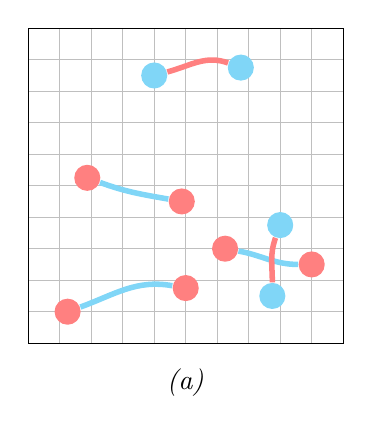
\begin{tikzpicture}
      \drawquasigrid
      \node at (2, -.5) {\emph{(a)}};
    \end{tikzpicture}
    \hspace{1cm}
    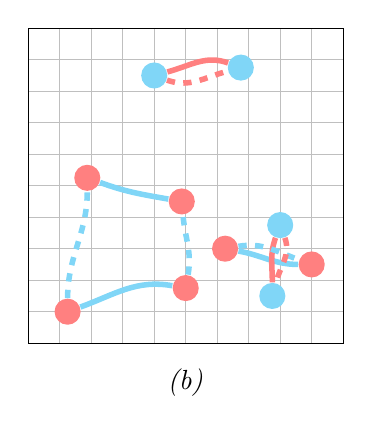
\begin{tikzpicture}
      \drawquasigrid
      \draw[dashed, blueline] (N1) to[out=90, in=270] (N5);
      \draw[dashed, blueline] (N2) to[out=80, in=275] (N6);
      \draw[dashed, blueline] (N3) to[out=10, in=160] (N4);
      \draw[dashed, redline] (N7) to[out=-20, in=195] (N8);
      \draw[dashed, redline] (N9) to[out=290, in=75] (N10);
      \node at (2, -.5) {\emph{(b)}};
    \end{tikzpicture}
    \hspace{1cm}
    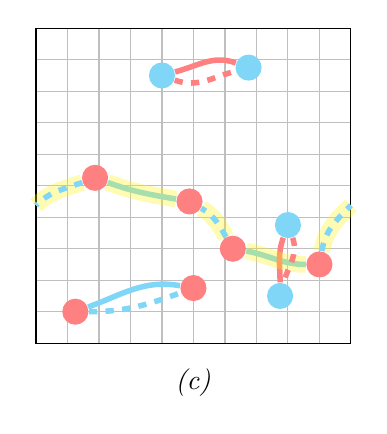
\begin{tikzpicture}
      \drawquasigrid
      \draw[yellow, line width=6, opacity=.3] (N3) to[in=180, out=-10] (N4);
      \draw[yellow, line width=6, opacity=.3] (N5) to[in=170, out=-20] (N6);
      \draw[yellow, line width=6, opacity=.3] (N3) to[out=120, in=-30] (N6);
      \draw[yellow, line width=6, opacity=.3] (N5) to[out=200, in=45] (0, 1.75);
      \draw[yellow, line width=6, opacity=.3] (N4) to[out=80, in=225] (4, 1.75);
      \draw[dashed, blueline] (N1) to[out=0, in=200] (N2);
      \draw[dashed, blueline] (N3) to[out=120, in=-30] (N6);
      \draw[dashed, blueline] (N5) to[out=200, in=45] (0, 1.75);
      \draw[dashed, blueline] (N4) to[out=80, in=225] (4, 1.75);
      \draw[dashed, redline] (N7) to[out=-20, in=195] (N8);
      \draw[dashed, redline] (N9) to[out=290, in=75] (N10);
      \node at (2, -.5) {\emph{(c)}};
    \end{tikzpicture}
    \caption{The quasiparticle picture of stabilizer measurements. Anticommuting stabilizers behave as anyons (circles), where a chain of errors (lines) creates a pair of anyons. Figure (b) shows a successful decoding of (a). Figure (c) shows a pairing that resulted in a correction operator that is in a different class as the error operator, which acquires a logical error. (Figure inspired by \cite{naomi})}\label{fig:quasiparticle}
  \end{figure}
  
Figure \ref{fig:quasiparticle}a shows the quasiparticle representation of the errors suffered in Figure \ref{sf:fig_degenerate}a, which has suffered Z (blue lines) and X errors (red lines). The corresponding anyons can either be of the star type (red circle) or plaquette type (blue circle). Figure \ref{fig:quasiparticle}b shows a successful decoding. Note that here not all pairs are correctly identified, but the resulting loop still is in the same class of operators. In figure \ref{fig:quasiparticle}c the correction has failed as the resulting loop in the correction is in a difference class compared to the error. As the loop still commutes with the stabilizer, no error can be detected, but the encoded qubit has acquired a logical error.


\section{Union-Find}\label{sec:UFdecoder}

The Union-Find decoder is a new fast decoding algorithm for topological codes to correct for Pauli errors, erasure errors, and the combination of both errors. The worst-case complexity of the algorithm is $\m{O}(n\alpha(n))$, where $n$ is the number of physical qubits and $\alpha$ is the inverse of Ackermann's function, which is very slowly growing, and is proven that $a(n)\leq 3$ for any practical amount of qubits.

Many types of decoding algorithms have been developed for the surface code, including the optimal decoder and the MWPM-decoder. Most of these decoders run at best in polynomial time, which is often considered efficient, but in practice even quadratic or cubic complexity is likely too slow to correct errors faster than they accumulate in a quantum device. Furthermore, any speed-up of the decoder will indirectly lead to a reduction of the noise strength, as a shorter time between two rounds of correction allows for fewer errors to appear. To this end, a new decoding algorithm named the \emph{Peeling decoder} has been developed that can solve errors over the erasure channel with a linear time complexity. The \emph{Union-Find} decoder is an extensions that additionally solves for Pauli errors. We will explore both algorithms in the coming sections and perform analyses on their complexities. 

\subsection{The Peeling decoder}
he Peeling decoder acquired its name by the nature of its behavior of sequentially \emph{peeling} from some tree of qubit-edges until the correction operator is left \cite{delfosse2017linear}. The scope of this decoder is limited to \emph{erasure} errors, or errors suffered through the erasure channel. Recall from equation \ref{qec:eq:erasure} that in an erasure, each qubit is erased from the system independently with probability $p_E$. Such a loss can be detected and the missing qubit is replaced by a totally mixed state of equation \ref{qec:eq:mixstate}, which can be interpreted as the original state that suffers from a Pauli error $I$, $X$, $Y$ or $Z$ chosen uniformly at random. Due to this uniform distribution, the primal and dual lattices of the surface code can be decoded separately from each other. The erased edges of graph $G_v(V,E_v)$ and $G_f(V,E_f)$ (see section \ref{sec:toricgraph}) suffer uniformly distributed $\{I,X\}$ and $\{I,Z\}$, respectively. We will consider $G_v(V,E_v)$ and simplify its notation to $G(V,E)$. 

We describe the decoding process of the primal lattice $G(V,E)$ and denote the set of lost qubits by $\gls{erasure}\subseteq E$. The set of Pauli errors within the erasure is $P_\m{E} = \{X_1,...X_m\}$. Error detection is performed in the same way as Pauli errors; by measuring the set of star operators or vertices $V$, which returns a set of nontrivial syndrome measurements $\sigma \subseteq V$. The decoder of an erasure error is thus provided with the extra information $\m{E}$, the subset of erased qubit locations, next to $\sigma$. 
\begin{lemma}\label{lem:peelinguni}
  For an erasure $\m{E} \subseteq E$ with uniformly distributed Pauli errors $P_\m{E}$ on a surface code, and a measured syndrome $\sigma$, any error  $\tilde{P}_\m{E}$ that produces $\sigma$ in a measurement is the most likely set of errors. 
\end{lemma}
\begin{proof}
  For the coset $\tilde{P}_\m{E}\cdot S$, where $\tilde{P}_\m{E}$ is some Pauli error caused by an erasure and $S$ is a set of stabilizers that act trivially on the codespace, the most likely configuration is the one that maximizes probability $\mathbb{P}(\tilde{P}_\m{E}\cdot S|\m{E},\sigma)$, where $\m{E}$ and $\sigma$ are known. This probability is proportional to $|\tilde{P}_\m{E}\cdot S \cap\m{E}|$. But since all qubits in $\m{E}$ suffer a Pauli error and this error is uniformly distributed, all configurations of $\tilde{P}_\m{E}$ have equal probability. 
  % Let $\m{E}\subseteq E$ be an erasure, a set of qubits on which an erasure error occurs, and let $\sigma \subseteq \m{S}$ be the measured error syndrome, the subset of the stabilizer generator group $\m{S}$, that anticommute with the erasure errors. In the absence of Pauli errors, all errors $P$ must lie inside the erasure.Therefore, for any measured syndrome, the path of errors must also be in the erasure, which can be denoted by $P\subseteq \m{E}$. As a result of this, in the case that the Pauli errors within the erasure are uniformly distributed, any error $\tilde{P}\subseteq\m{E}$ that produces the syndrome $\sigma$ is the most likely coset. 
\end{proof}

Consequently, if the error set $\tilde{P}_\m{E}$ is applied as the correction operator $C=\tilde{P}_\m{E}$, the resulting decoder is a \emph{maximum likelihood decoder}. In order to find $C$, we now do not try to find paths within $\m{E}$ that pair the syndrome vertices of $\sigma$, but rather try to recursively shrink the set of edges on which a decision is to be made. 
\begin{definition}\label{def:boundaryofedges}
  The boundary or support of a set of edges $\gls{boundary}(\tilde{E})$ denotes the set of vertices $\tilde{V}$ that supports all edges $e\in \tilde{E}$.
\end{definition}
\begin{definition}\label{def:forest}
  A spanning forest $F_{\tilde{E}}$ is a maximal subset of edges of $\tilde{E}$ that contains no cycles and $\mathscr{B}(F_{\tilde{E}}) = \mathscr{B}(\tilde{E})$.
\end{definition}
The first step in this is to produce $\gls{forest}$ inside $\m{E}$, where all syndrome vertices $\sigma$ are included in the support. Hence if $\m{E}$ is a connected graph, then $F_\m{E}$ is connected \emph{acyclic} graph. Such a forest can be found in linear time by either a depth-first search or breadth-first search of the $\m{E}$. Next, the decoder further reduces the size of the spanning forest $F_\m{E}$ by sequentially peeling edges from the tree, while constructing the correction set $\gls{correctionset}$, initiated as an empty set. The decoder loops over all edges in $F_\m{E}$, each time picking a \emph{leaf} edge $e = \{u,v\}$, connected to the forest by only one vertex $v$, removing the leaf edge from $F_\m{E}$. If the so-called \emph{pendant} vertex $u\in\sigma$, remove $u$ from $\sigma$, and $e$ is added to $\m{C}$ and the vertex $v$ is \emph{flipped}, such that $v$ is added to $\sigma$ if $v \notin \sigma$, and removed from $\sigma$ if $v\in\sigma$.  If $u\notin\sigma$, the edge $e$ is simply removed from $F_\m{E}$ (see algorithm \ref{algo:peel}). On account of these rules, edges on a branch that had a syndrome vertex as a leaf will continuously be added to $\m{C}$ until it encounters another syndrome vertex, creating a correction path between a syndrome pair. The dual lattice can be decoded in a similar way.
\begin{definition}
  The \emph{Pauli product} of a set of edges $\tilde{E}$ is the defined as the product of Pauli operators on each of the edges in the set
  \begin{equation}
    \gls{pauliproduct}(\tilde{E}) = \prod_{e\in \tilde{E}} \hat{P}_e,
  \end{equation}
  where the Pauli operator $\hat{P}$ corresponds to $X$ if $\tilde{E}\subseteq E_v$ and $Z$ if $\tilde{E}\subseteq E_f$. 
\end{definition}
\begin{algo}[algotitle=Peeling decoder (adapted from \cite{delfosse2017linear}), label=algo:peel]
  \begin{algorithm}[H]
    \KwData{A graph $G = (V,E)$, an erasure $\m{E} \subseteq E$ and syndrome $\sigma \subseteq V$}
    \KwResult{Correction $C$}
    \BlankLine
    construct a spanning forest $F_\m{E} \subseteq\m{E}$\;
    initialize $\m{C}$ by $\m{C} = {\emptyset}$\;
    \While{$F_\m{E} \neq \emptyset$}{
    pick a leaf edge $e = {u,v}$ with pendant vertex $u$, remove $e$ from $F_\m{E}$ \;
    \If{$u \in \sigma$}{
      add $e$ to $\m{C}$, remove $u$ from $\sigma$ and flip $v$ in $\sigma$}
    \Else{do nothing}
    }
    \KwRet{$C = \prod_{e\in \m{C}} X_e$}
  \end{algorithm}
\end{algo}
The spanning forest $F_\m{E}$ can be constructed in linear time. Also, the loop over the forest can be operated in linear if the list of leaves is pre-computed and updated during the loop. Thus the Peeling decoder has a linear time complexity in the size of the erasure $\m{O}(\abs{\m{E}})$ and therefore also in the number of qubits $\m{O}(n)$. Now, the structure of the forest $F_\m{E}$ is very dependent on from which vertex the DFS is started, and proof is required that any forest of $\m{E}$ is valid. Also, we show that for each forest, the peeling process returns the same correction.

\begin{lemma}\label{lem:anyforest}
  For any choice of $F_\m{E}$, there exists a subset $\m{C}\subseteq F_\m{E}$ such that $\mathscr{P}(\m{C})$ corrects the syndrome set $\sigma$.
\end{lemma}
\begin{proof}
  There exists a subset of edges $\tilde{E} = \{e_1,...,e_m\} \subseteq F_\m{E}$ such that $\mathscr{P}(\tilde{E})$ has a syndrome $\sigma$. By the definition of the forest $F_\m{E}$, adding another edge $e' \in F_\m{E} \vartriangle \m{E}$ creates a cycle $\gamma' \subseteq F_\m{E} \cup \{e_i\}$, where $\vartriangle$ denotes the symmetric difference between two sets. Now $\tilde{E}$ can be replaced by $\tilde{E}'=\tilde{E}\vartriangle\gamma'$ whose Pauli product $\mathscr{P}(\tilde{E}')$ has the same syndrome $\sigma$, as $\vartriangle$ augments the matching path between syndromes within $\gamma'$. Now, any edge $e_r\in \gamma' \notin \tilde{E}'$ can be removed from to create a new forest $F_\m{E}'=F_\m{E} \cup \{e_i\}\setminus e_r|e_r \neq e'$. For any cycle that exists from larger than 3 elements, $e_r$ must exist. Thus the Pauli product of subset $\tilde{E}' \subseteq F_\m{E}'\subseteq \m{E}$ is also a valid error with syndrome $\sigma$, and $\mathscr{P}(\tilde{E}')$ corrects $\sigma$. This can be done any number of times, thus every $F_\m{E}$ is valid.   
\end{proof}
\begin{lemma}\label{lem:peelingfe}
  The output correction set $\m{C}$ from the Peeling decoder is only dependent on spanning tree $F_\m{E}\subseteq\m{E}$, and not on the peeling process. 
\end{lemma}
\begin{proof}
   For each $F_\m{E}$, the outcome $\m{C}$ after peeling is unique and independent from the order of peeling. If there exists two subsets $\m{C}$ and $\m{C}'$, applying both $\mathscr{P}(\m{C})\mathscr{P}(\m{C}')$ yields the empty syndrome set $\sigma=\emptyset$, which means that either $\mathscr{P}(\m{C})\mathscr{P}(\m{C}')$ is a cycle or $\m{C}=\m{C}'$. Since $F_\m{E}$ has no cycles it means that $m{C}$ must be unique within $F_\m{E}$.
\end{proof}

\tikzset{
  anyon/.style={circle, fill=OrangeRed, minimum size=.2cm, inner sep=0},
  erasure/.style={NavyBlue, very thick},
  correction/.style={Green, very thick},
  description/.style={align=#1, text width=4cm},
  description/.default={left},
  error/.style={text=black, pos=0.5}
  }

\begin{figure}
  \centering
  \begin{tikzpicture}[on grid, scale=0.8]
    \node at (0,4) {a)};
    \draw[step=1cm,gray,thin] (0.1,0.1) grid (3.9,3.9);
    \draw[erasure] (1,1) -- (2,1) node[error]{$X$} -- (3,1) -- (3,2) -- (2,2) -- (1,2) -- cycle node[error]{$X$};
    \draw[erasure] (1,2) -- (1,3) -- (2,3) node[error]{$X$} -- (2,2);
    \node[description={center}] at (2, -.5) {initial state};

    \begin{scope}[shift={(6,0)}]
      \node at (0,4) {b)};
      \draw[step=1cm,gray,thin] (0.1,0.1) grid (3.9,3.9);
      \draw[erasure] (1,1) -- (2,1) node[anyon]{} -- (3,1) -- (3,2) -- (2,2) -- (1,2) node[anyon] (a) {} -- cycle;
      \draw[erasure] (a) -- (1,3) node[anyon]{} -- (2,3) node[anyon]{}-- (2,2);
      \node[description={center}] at (2, -.5) {identify syndrome};
    \end{scope}

    \begin{scope}[shift={(12,-.5)}]
      \draw[thin] (0,4) -- ++(.5,0) ++(.5,0) node[anchor=west]{normal edge};
      \draw[thin] (0,3) -- ++(.5,0) node[error]{$X$} ++(.5,0) node[anchor=west]{Pauli error};
      \draw[erasure] (0,2) -- ++(.5,0) ++(.5,0) node[anchor=west, text=black]{erased edge};
      \draw[thin] (0,1) -- ++(.5,0) node[anyon,pos=.5]{} ++(.5,0) node[anchor=west]{syndrome};
      \draw[correction] (0,0)   -- ++(.5,0) ++(.5,0) node[anchor=west,text=black]{correction edge};
    \end{scope}

    \begin{scope}[shift={(0,-6)}]
      \node at (0,4) {c)};
      \draw[step=1cm,gray,thin] (0.1,0.1) grid (3.9,3.9);
      \draw[erasure] (1,3) node[anyon]{} -- (2,3) node[anyon]{} -- (2,2) -- (1,2) node[anyon]{} -- (1,1) -- (2,1) node[anyon]{} -- (3,1) -- (3,2);
      \node[description={center}] at (2, -.5) {construct $F_{\varepsilon}$};
    \end{scope}

    \begin{scope}[shift={(6,-6)}]
      \node at (0,4) {d)};
      \draw[step=1cm,gray,thin] (0.1,0.1) grid (3.9,3.9);
      \draw[erasure] (1,3) node[anyon]{} -- (2,3) node[anyon]{} -- (2,2) -- (1,2) node[anyon]{} -- (1,1) -- (2,1) node[anyon](a){};
      \draw[erasure, dashed] (a) -- (3,1) node[pos=0, below, text=black]{$v$} node[pos=0.5, above]{$e$} node[pos=1, below, text=black]{$u$};
      \node[description={center}] at (2, -.5) {peel $e=(u,v), u \notin \sigma$};
    \end{scope}

    \begin{scope}[shift={(12,-6)}]
      \node at (0,4) {e)};
      \draw[step=1cm,gray,thin] (0.1,0.1) grid (3.9,3.9);
      \draw[erasure] (1,3) node[anyon]{} -- (2,3) node[anyon]{} -- (2,2) -- (1,2) node[anyon]{} -- (1,1);
      \draw[erasure, dashed] (1,1) node[below, text=black]{$v$} -- (2,1) node[anyon]{} node[pos=0.5, above]{$e$} node[below, text=black]{$u$};
      \node[description={center}] at (2, -.5) {peel $e=(u,v), u \in \sigma$};
    \end{scope}

    \begin{scope}[shift={(0,-12)}]
      \node at (0,4) {f)};
      \draw[step=1cm,gray,thin] (0.1,0.1) grid (3.9,3.9);
      \draw[erasure] (1,3) node[anyon]{} -- (2,3) node[anyon]{} --  (2,2) -- (1,2) node[anyon]{} -- (1,1) node[anyon](a){};
      \draw[correction] (a) node[below, text=black]{$v$} -- (2,1) node[pos=0.5, above]{$e$} node[below, text=black]{$u$};
      \node[description={center}] at (2, -.5) {flip $u,v$, add $e$ to $C$};
    \end{scope}

    \begin{scope}[shift={(6,-12)}]
      \node at (0,4) {g)};
      \draw[step=1cm,gray,thin] (0.1,0.1) grid (3.9,3.9);
      \draw[correction] (1,3) -- (2,3) node[error]{$X$} (2,1) -- (1,1) node[error]{$X$} -- (1,2) node[error]{$X$};
      \node[description={center}] at (2, -.5) {apply correction set $C$};
    \end{scope}

    \begin{scope}[shift={(12,-12)}]
      \node at (0,4) {h)};
      \draw[step=1cm,gray,thin] (0.1,0.1) grid (3.9,3.9);
      \node[description={center}] at (2, -.5) {end state};
    \end{scope}
  \end{tikzpicture}
  \caption{Schematic representation of the Peeling decoder. On an erasure $\m{E}\subset E$ (a), there may be some Pauli errors $P\subset \m{E}$ that anticommutes with some stabilizer measurements (b) that is identified as the syndrome $\sigma$. The first step is to construct a spanning forest $F_\m{E}\subset \m{E}$, a fully connected acyclic graph. Next the decoder sequentially removes leaf edges $e=(u,v)$ from the forest that connect to the forest via only one vertex $v$. If $u\in\sigma$ (e), remove $u$ from $\sigma$, flip $v$ in $\sigma$ and the edge $e$ is added to the correction set $C$ (f). If $u \notin \sigma$, move on the the next leaf. After applying the correction set $C$ (g), all errors on the lattice commutes with the stabilizers, potentially solving the error (h).}
\end{figure}

The peeling decoder will always output some correction $C$ such that $CP_\m{E}$ commutes with the stabilizer, given a set of nontrivial stabilizer measurements $\sigma$. This is proven by the previous lemmas. Finally, we will prove that this is true for any erasure $\m{E}\subseteq E$. 
\begin{theorem}\label{eq:anyevenparity}
  For any connected graph that suffered some erasure $\m{E}\subseteq E$ with pauli error $P_\m{E}$, if the parity of the number syndrome vertices within the graph is even, applying the Peeling decoder (algorithm \ref{algo:peel}) will produce a correction $\m{C}\subseteq \m{E}$ such that $\mathscr{P}(\m{C})P_\m{E}=CP_\m{E}$ commutes with the stabilizer.
\end{theorem}
\begin{proof}
  Consider a spanning forest $F_\m{E}$ containing $n_\sigma$ syndrome vertices. The forest is being stripped by the Peeling decoder on the leaf edge $e = (u,v)$, where the vertex $v$ is the pendant vertex. If $u\notin\sigma$, $e$ is simply removed from $F_\m{E}$ and $n_\sigma$ is unaltered. If $u\in\sigma$, $u$ is removed from $\sigma$ such that $n_\sigma'= n_\sigma -1$. Vertex $v$ is now flipped in $\sigma$, meaning that if $v\in\sigma$, it is removed and $n_\sigma'= n_\sigma -2$, or if  $v\notin\sigma$, it is added and $n_\sigma'= n_\sigma$. After peeling it must be that $n_\sigma=0$, from which follows that all erasures with \emph{even} parity can be solved. 
\end{proof}

\begin{definition}\label{def:cluster}
  A cluster $C$ is a subset of an erasure $\m{E}$, such that the edges of $C$ form a connected graph. 
\end{definition}
\begin{lemma}\label{lem:singlecluster}
  An edge $e$ can only belong to a single cluster. A vertex $v$ can only be in the boundary of a single cluster $\mathscr{B}(C)$. 
\end{lemma}
\begin{proof}
  If there exists some edge $e$ that belongs to two clusters $C_i, C_j$, they are connected via $e$. Per definition \ref{def:cluster} clusters $C_i, C_j$ must be a single cluster. The same is true for some vertex $v$ that belongs to both $\mathscr{B}(C_i)$ and $\mathscr{B}(C_j)$. 
\end{proof}
For only erasure noise, all erasures must have even parity as all errors $P_\m{E}$ and thus all syndromes $\sigma \in \mathscr{B}(\m{E})$, which is why erasure noise is the scope of the Peeling decoder. As other types of noise are added, modifications to the Peeling decoder are needed, as we will see later. Finally, we note that an erasure $\m{E}$ may not be a single subset of connected edges, but rather many connected subsets, denoted by $C_i$. This does not change anything in the decoder, as the peeling algorithm will pass every edge once, which is ensured by lemma \ref{lem:singlecluster}. Each cluster $C_i$ returns its own connected acyclic $F_{C_i}$ that can be peeled separately from each other. 
\begin{theorem}
  The Peeling decoder (algorithm \ref{algo:peel}) is a linear-time maximum likelihood decoder for erasures up to $d-1$ qubits, where $d$ is the minimum distance of the code. 
\end{theorem}
\begin{proof}
  If the erasure $\m{C}$ does not support a subset of edges that is equivalent to some logical operator $L=\mathscr{P}(\tilde{E})|\tilde{E}\subseteq\m{E}$, the product of the error and correction $CP_\m{E}$ cannot lead to a logical error, as $\m{C}\subseteq \m{E}$. Furthermore, on account of lemmas \ref{lem:peelinguni}, \ref{lem:anyforest} and \ref{lem:peelingfe}, any correction set $\m{C}\subseteq F_\m{E}$ is the most likely correction. Thus for any erasure pattern up to $d-1$ qubits, the Peeling decoder is a linear-time maximum likelihood decoder. 
\end{proof}

\subsubsection{Bounded surfaces}
For bounded surfaces such as the planar code (sec \ref{sec:surface_planar}), the peeling decoder needs some small alterations. Let us again only consider the primal lattice which is now denoted by $G = (V_\iota\cup V_{\delta} \cup V_{\omega}, E_\iota \cup E_{\delta})$. Syndrome measurements on such a graph are only supported by $\sigma \subseteq V_\iota\cup V_\delta$, as $V_\delta$ are \emph{open} vertices that only exist to support boundary edges $E_\delta$, and do not refer to some stabilizer generator or physical measurement. The missing information on $V_\delta$ makes it impossible to apply the pendant vertex rule at these vertices. To ensure that the peeling algorithm does not become stuck, we add the restriction for the pendant vertex $u \notin V_\delta$. Furthermore, the construction of the forest $F_\m{E}$ requires an additional alteration.
\begin{lemma}
  Two vertices $u,v$ within a forest $F_\m{E}$ that satisfy $u\in V_\delta, v \in V_\delta$ is equivalent to a cycle in $F_\m{E}$. 
\end{lemma}
\begin{proof}
  If there are an even number of vertices in a forest $F_\m{E}$ that are supported by $V_\delta$, it means that there are a number of unique paths within $F_\m{E}$ that lead from a element of $V_\delta$ to another element of $V_\delta$. Such a path is equivalent to some $\delta$-operators and commutes with the stabilizer. Hence, it cannot be caused by some detected error which anticommutes with the stabilizer.
\end{proof}
Due to this, we ensure that each forest $F_\m{E}$ can only support a maximum of 1 element of $V_\delta$. The forests are grown starting from vertices of the set $V_\delta$, and the algorithm is completed by a DFS same as before with the additional requirement. Note that now for every cluster, more than one connected acyclic forests may be formed, dependent on the number edges connected to the boundary. But yet every forest can still be peeled independently, as every edge can only be peeled once. 

\begin{algo}[algotitle=Peeling decoder for bounded surfaces (adapted from \cite{delfosse2017linear}), label=algo:peelbound]
  \begin{algorithm}[H]
    \KwData{A graph $G = (V\cup V_\delta,E)$, an erasure $\m{E} \subseteq E$ and syndrome $\sigma \subseteq V$}
    \KwResult{Correction $C$}
    \BlankLine
    construct a spanning forest $F_\m{E}\subseteq\m{E}$ with seed $V_\delta$\;
    initialize $\m{C}$ by $\m{C} = {\emptyset}$\;
    \While{$F_\m{E} \neq \emptyset$}{
    pick a leaf edge $e = {u,v}$ with pendant vertex $u\notin V_\delta$, remove $e$ from $F_\m{E}$ \;
    \If{$u \in \sigma$}{
      add $e$ to $\m{C}$, remove $u$ from $\sigma$ and flip $v$ in $\sigma$}
    \Else{do nothing}
    }
    \KwRet{$C = \prod_{e\in \m{C}} X_e$}
  \end{algorithm}
\end{algo}

\begin{figure}
    \centering
    \begin{tikzpicture}[on grid, scale=0.8]
      \node at (-.5,4) {\emph{(a)}};
      \draw[step=1cm,gray,thin] (0.1,0) grid (3.9,4);
      \draw[erasure] (0.1,1) -- (1,1)  -- (2,1)  node[error]{$X$} -- (2,2) -- (2,3) -- (1,3)  -- (1,2) node[error]{$X$}  -- (0.1,2)  node[error]{$X$} (1,1) -- (1,2) -- (2,2);
      \draw[erasure] (3.9,4) -- (3,4)  node[error]{$X$} -- (3,3)  -- (3,2)  node[error]{$X$}  -- (3.9,2) (2,3) -- (3,3) -- (3.9,3);
      \node[description={center}] at (2, -.5) {initial state};
  
      \begin{scope}[shift={(6,0)}]
        \node at (-.5,4) {\emph{(b)}};
        \draw[step=1cm,gray,thin] (0.1,0) grid (3.9,4);
        \draw[erasure] (0.1,1) -- (1,1) node[anyon]{} -- (2,1) node[anyon]{} -- (2,2) -- (2,3) -- (1,3) node[anyon]{} -- (1,2)  -- (0.1,2) (1,1) -- (1,2) -- (2,2);
        \draw[erasure] (3.9,4) -- (3,4) node[anyon]{} -- (3,3) node[anyon]{} -- (3,2) node[anyon]{}  -- (3.9,2) (2,3) -- (3,3) -- (3.9,3);
        \node[description={center}] at (2, -.5) {identify syndrome};
      \end{scope}
  
      \begin{scope}[shift={(12,-.5)}]
        \draw[thin] (0,4) -- ++(.5,0) ++(.5,0) node[anchor=west]{normal edge};
        \draw[thin] (0,3) -- ++(.5,0) node[error]{$X$} ++(.5,0) node[anchor=west]{Pauli error};
        \draw[erasure] (0,2) -- ++(.5,0) ++(.5,0) node[anchor=west, text=black]{erased edge};
        \draw[thin] (0,1) -- ++(.5,0) node[anyon,pos=.5]{} ++(.5,0) node[anchor=west]{syndrome};
        \draw[correction] (0,0)   -- ++(.5,0) ++(.5,0) node[anchor=west,text=black]{correction edge};
      \end{scope}

      \begin{scope}[shift={(0,-6)}]
        \node at (-.5,4) {\emph{(c)}};
        \draw[step=1cm,gray,thin] (0.1,0) grid (3.9,4);
        \draw[erasure] (0.1, 2) -- (1,2) -- (1,1) node[anyon]{} -- (2,1) node[anyon]{} -- (2,2) -- (2,3) -- (1,3) node[anyon]{};
        \draw[erasure] (3.9,4) -- (3,4) node[anyon]{} -- (3,3) node[anyon]{} -- (3,2) node[anyon]{};
        \node[description={center}] at (2, -.5) {construct $\m{T}_\m{R}$};
      \end{scope}

      \begin{scope}[shift={(6,-6)}]
        \node at (-.5,4) {\emph{(d)}};
        \draw[step=1cm,gray,thin] (0.1,0) grid (3.9,4);
        \draw[correction] (0.1, 2) -- (1,2) node[error]{$X$} -- (1,1) node[error]{$X$} (2,1)  -- (2,2) node[error]{$X$} -- (2,3) node[error]{$X$} -- (1,3) node[error]{$X$};
        \draw[correction] (3.9,4) -- (3,4) node[error]{$X$} (3,3) -- (3,2) node[error]{$X$};
        \node[description={center}] at (2, -.5) {apply correction $\n{P}(\m{C})$};
      \end{scope}

      \begin{scope}[shift={(12,-6)}]
        \node at (-.5,4) {\emph{(e)}};
        \draw[step=1cm,gray,thin] (0.1,0) grid (3.9,4);
        \path (1,1) -- (2,1) node[error]{$X$} -- (2,2) node[error]{$X$} -- (2,3) node[error]{$X$} -- (1,3) node[error]{$X$} -- (1,2) node[error]{$X$} -- (1,1) node[error]{$X$};
        \node[description={center}] at (2, -.5) {end state};
      \end{scope}

    \end{tikzpicture}
    \caption{Schematic visualization of the Peeling decoder on a surface with boundaries. On an erasure $\m{R}\subset \m{E}$ (a), there may be some Pauli errors $\m{E}_\m{R} \subset \m{R}$ that anticommutes with some stabilizer measurements (b) that is identified as the syndrome $\sigma$. (c) The forest $\m{T}_\m{R}$ now has the extra constriction that it can only support single element of $\m{V}_\delta$, the open vertices, and peeling is only allowed on pendant vertices $v\notin \m{V}_\delta$. (d) After peeling, the correction $\n{P}(\m{C})$ is outputted and can be applied to correct error. (e) The end state is now a cycle of errors, which commutes with the stabilizer. This is not a feature of the Peeling decoder, but is just an example.}
  \end{figure}




\subsection{Union-Find data structure}
The Union-Find data structure, also known as the \emph{disjoint-set} data structure \cite{tarjan1975efficiency}, is the data structure that is crucial for the near linear complexity of the Union-Find decoder. In this section, we describe the data structure and analyse its complexity. 

The disjoint-set data structure consists of two types of instructions for manipulating a set of elements partitioned into a number of disjoint subsets, which are non-overlapping. These instructions provide near-constant-time operations to determine whether elements are in the same set, and to merge sets if that is not the case. 
\begin{itemize}
  \item $\codefunc{Find}(x)$ computes the unique set containing the element $x$
  \item $\codefunc{Union}(A,B)$ combines sets $A$ and $B$ into a new combined set
\end{itemize}
We first show that a very simple implementation runs in $\m{O}(n^2)$ time. Applying the \emph{union by weight} rule, this is reduced to $\m{O}(n \log n)$. Combined with the \emph{Path compression} rule, the overall complexity is $\m{O}(n \alpha (n))$, where $\alpha$ is the inverse of Ackermann's function. The original proof \cite{tarjan1975efficiency} was further reinforced by subsequent publications \cite{tarjan1979class,tarjan1984worst} and was proven to be optimal \cite{fredman1989cell}. In this thesis, we will follow a simplified approach, where the \emph{union by weight} rule is replaced by a different by similar \emph{union by rank} rule \cite{kozen1992design}. Later Tarjan and also other sources used this to cast this analysis in terms of potential functions \cite{tarjan1999handout, harfst2000potential, cormen2009introduction}. Another approach is provided by \cite{seidel2005top}, where the upper bound is computed via a top-down method. 


\subsubsection{Simple implementation}
A simple implementation of the instructions would be to store for each set $X$ a list $l_X$ of all the elements it contains, and a pointer to $l_X$ at all elements $x\in l_X$, which is called the \emph{linked-list} representation. The function $\codefunc{find}(x)$ simply returns the list $l_X$, which represents the set. After a call to $\codefunc{Union}(X, Y)$, all elements of $l_Y$ are appended to $l_X$, and the pointers of all elements $y\in Y$ are updated. This takes $\m{O}(m)$ operations, where $m=|l_Y|$ the number of elements. In a system of $n$ elements, there may be a maximum of $n-1$ calls to \codefunc{Union}. As the $i$\textsuperscript{th} call involves sets $|l_X|=1$ and $|l_Y|=i$, the number of updates is 
\begin{equation}
  \sum_{i=1}^{n-1} i = \m{O}(n^2),
\end{equation}
where each \codefunc{Union} operation has on average $\m{O}(n)$ updates. 

\subsubsection{Union by weight}
In the above case, we assume in each \codefunc{Union} the worst case where a larger list is appended to a smaller list, and the pointers of the largest list must be updated. Suppose that each list $l_X$ additionally stores the length of the list itself, which can be easily maintained, it can be set as a rule to always append the smaller list to the larger list. With this simple rule, the complexity of the Union-Find algorithm can be reduced to $\m{O}(n \log n)$. 

\begin{theorem}
  A sequence of \codefunc{Union} and \codefunc{Find} operations on $n$ initial single element disjoint sets using the weighted union rule takes $\m{O}(n \log n)$ time. 
\end{theorem}
\begin{proof}
  Consider a set $X$ with list $l_X$ that undergoes a sequence of \codefunc{Union} and \codefunc{Find} operations. The first time all pointers in $l_X$ are updated, the resulting set must have at least 2 elements. Similarly, the next time all pointers are updated, the resulting set must have at least 4 elements due to the weighted union rule. With system size $n$, any initial set $X$ can be updated at most $\log n$ times, where the update size is proportional to $n$. Hence the sequence takes $\m{O}(n \log n)$ time. 
\end{proof}

\subsubsection{Disjoint-set trees}
The pointer update in each set during a \codefunc{Union} can be minimized by a different representation of the Union-Find data structure, where each set is represented by a \emph{rooted tree}. Each member has a pointer to its parent, and the root of the tree points to itself, and is the representative element of the cluster. Function \codefunc{Find} is now performed by following the parent pointers until the root of the tree, and $\codefunc{Union}$ points one root towards another, such that there is only one single root that is the representative element. Each call to $\codefunc{Union}(r_x,r_y)$ is preceded by calls to $r_x=\codefunc{Find}(x)$ and $r_y=\codefunc{Find}(y)$ to find their respective roots and to link their trees if $r_x \neq r_y$. 

\tikzstyle{lw1}=[line width=1]
\tikzstyle{fnode}=[draw, circle, minimum size=0.65cm, inner sep=0, lw1]

\begin{figure}[]
  \centering
  \begin{tikzpicture}[on grid]
    \node[fnode] at (0,0)(a){a};
    \node[fnode] at (0,1)(b){b};
    \node[fnode] at (0.75,2)(c){c};
    \node[fnode] at (1.5,1)(d){d};
    \node[fnode] at (3,0)(e){e};
    \node[fnode] at (3,1)(f){f};
    \node[fnode] at (3,2)(g){g};
    \draw[lw1, ->] (a) -- (b);
    \draw[lw1, ->] (b) -- (c);
    \draw[lw1, ->] (d) -- (c);
    \draw[lw1, ->] (e) -- (f);
    \draw[lw1, ->] (f) -- (g);
    \draw[lw1, ->] (c) .. controls +(0.75,1) and +(-0.75,1) .. (c);
    \node at (1.5,-1) {(a)};

    \begin{scope}[shift={(6,-1)}]
      \node at (1.5,0) {(b)};
      \node[fnode] at (0,0)(a2){a};
      \node[fnode] at (0,1)(b2){b};
      \node[fnode] at (0.75,2)(c2){c};
      \node[fnode] at (1.5,1)(d2){d};
      \node[fnode] at (2.75,1)(e2){e};
      \node[fnode] at (2.75,2)(f2){f};
      \node[fnode] at (1.75,3)(g2){g};
      \draw[lw1, ->] (a2) -- (b2);
      \draw[lw1, ->] (b2) -- (c2);
      \draw[lw1, ->] (d2) -- (c2);
      \draw[lw1, ->] (e2) -- (f2);
      \draw[lw1, ->] (f2) -- (g2);
      \draw[lw1, ->] (c2) -- (g2);
      \draw[lw1, ->] (g2) .. controls +(0.75,1) and +(-0.75,1) .. (g2);
    \end{scope}
  \end{tikzpicture}
  \caption{<caption>}
  \label{<label>}
\end{figure}

\subsubsection{Union by rank}

The \emph{union by weight} rule from the previous section can be implemented without any alteration. However, in the disjoint-set tree structure, a slightly different rule, \emph{union by rank}, can be implemented behaves similarly, but allows for a easier analysis of the complexity when combined with the \emph{path compression} rule, which is introduced in the next section. 

\begin{definition}
  The rank of a node $x$ is the maximum height of a subtree rooted in $x$. Let $R_t(x)$ denote the rank of node $x$ at time $t$. 
\end{definition}

The union by rank rule is then as follows: to apply $\codefunc{Union}(r_x,r_y)$, make the smaller-ranked root $R(r_x) < R(r_y)$ point to the larger; in case of a tie, also increase the rank of the new root by one. As long as a node $x$ has no parent, its rank can increase as other trees as pointed to itself. But as $x$ becomes a child of node $x$, the subtree rooted at $x$ become fixed and so does its rank. Any descendent $x$ of ancestor $y$ must thus always comply to $R(x)<R(y)$. 

\begin{lemma}\label{lem:rank1}
  Let $T_t(x)$ be the subtree rooted in node $x$ at time $t$, and let $|T_t(x)|$ denote the number of elements in the subtree, then if the weight by rank rule is implemented, it must be true that 
  \begin{equation}
    \abs{T_t(x)} \geq 2^{R_t(x)}
  \end{equation}
\end{lemma}
\begin{proof}
    \begin{equation*}
        R_t(x) = R_{t+1}(x) = R_{t+1}(y) - 1
    \end{equation*}
    \begin{equation*}
        \abs{T_{t+1}(y)} \geq abs{T_{t+1}(x)}
    \end{equation*}
    \begin{align*}
        \abs{T_{t+1}(y)} &= \abs{T_t(y)} + \abs{T_t(x)} \\
         &\geq 2^{R_t(x)} + 2^{R_t(x)} \\
         &= 2^{R_t(x)+1} \\
         &= 2^{R_{t+1}(y)}
    \end{align*}
\end{proof}


\begin{lemma}
    The maximum rank in all disjoint-set trees after a sequence calls to \codefunc{Find} and \codefunc{Union} in a system of $n$ elements is at most $\lfloor \log n \rfloor$. 
\end{lemma}
\begin{proof}
    By the previous lemma \ref{lem:rank1}, 
    \begin{equation*}
        n \geq \abs{T(x)} \geq 2^{R(x)}, 
    \end{equation*}
    Which leads to 
    \begin{equation*}
        \lfloor \log n \rfloor \geq R(x).
    \end{equation*}
\end{proof}

\begin{lemma}
    \begin{equation}
        \abs{\{x | R(u)=r \}} \leq \frac{n}{2^r}
    \end{equation}
\end{lemma}
\begin{proof}
    \begin{align*}
        n &\geq \abs{\underset{R(x)=r}{\bigcup} T(x)} \\
        &= \sum_{R(x)=r} \abs{T(x)} \\
        &\geq \sum_{R(x)=r} 2^r \\
        &= \abs{\{x | R(u)=r\}}\cdot 2^r
    \end{align*}
\end{proof}
% To keep track of the vertices of a cluster, it will be represented as a \emph{cluster tree}, where an arbitrary vertex of the cluster will be the root, and any other vertex will be a child of the root. Whenever an edge $(u,v)$ is fully grown, we will need to traverse the trees of the two vertices $u$ and $v$, and check whether they have the same root; whether they belong to the same cluster. If not, a merge is initiated by making the root of smaller cluster a child of the bigger cluster. These functions, \codefunc{find} and \codefunc{union} respectively, are part of the Union-Find algorithm (not to be confused with the Union-Find decoder) \cite{tarjan1975efficiency}.

% Within the Union-Find algorithm, two features ensure that the complexity of the algorithm is not quadratic. 1). With \textbf{path compression}, as we traverse a tree from child to parent until we reach the root, we make sure that each vertex encountered that we have encountered along the way is pointed directly to the root. This doubles the cost of the \codefunc{find}, but speeds up any future call to any vertex on the traversed path. 2). With \textbf{weighted union}, we make sure to always make the smaller tree a child of the bigger tree. This ensures that the overall length of the path to the root stays minimal. In order to make this happen, we just need to store the size of the tree at the root.



\subsection{Union-Find decoder}

In the context of the surface code, the vertices $v\in V$ are the elements and each disjoint set is the set over vertices that support a cluster $\mathscr{B}(C)$ (definitions \ref{def:boundaryofedges}, \ref{def:cluster}). It is redundant to additionally store the sets $C$ for edges, as it lemma \ref{lem:singlecluster} implies that if a vertex $v\in \mathscr{B}(C)$, that all edges support by $v$ satisfy $e \in C$. 

Note that while the nodes in the tree are equivalent to vertices $v \in V$, parent pointers in the disjoint-set tree structure are \emph{not} equivalent to edges $e\in E$. The edge set $E$ with its erasure subset $\m{E}\subseteq E$ and subsequently cluster $C\subseteq \m{E}$ and forest $F_C\subseteq C$ are related to physical qubits and the lattice structure of the surface code, whereas edges of the tree $\bound(C)$ exists to point towards the representative element at the root.

The Peeling decoder solves exclusively for erasure errors. To be able to compare with the MWPM decoder, or other types of decoders, Pauli noise must be included. To this end, we use the independent noise model of equations \ref{qec:eq:bitflip} and \ref{qec:eq:phaseflip}, which means that again we can consider the primal and dual lattices separately. These noise channels introduce extra Pauli errors $P_p$ such that not all Pauli errors are in the erasures $P\not\subseteq \m{E}$, where $P = P_p\triangle P_\m{E}$. This means also that not all syndromes are in the boundary of the erasure $\sigma \not\subseteq \mathscr{B}(\m{E})$ (definition \ref{def:boundaryofedges}), and odd parity clusters can occur. Per theorem \ref{eq:anyevenparity}, the Peeling decoder cannot solve for these errors, and needs some alteration.

To this end, an altered erasure $\bar{\m{E}}$ that contains only even-parity clusters can be constructed from the syndrome $\sigma$ in a pre-processing step that is dubbed \emph{syndrome validation}. The validated erasure $\bar{\m{E}}$ is compatible with the peeling decoder. To do this, we sequentially grow the clusters with an odd parity by an half-edge on the boundaries on the clusters. When two odd parity clusters meet, the merged cluster will have a even parity, and can now be solved by the peeling decoder. 
\begin{proposition}
  The Peeling decoder can be altered to additionally solve for Pauli errors by a pre-processing step that initializes some altered erasure $\bar{E}$, such that theorem \ref{eq:anyevenparity} is satisfied, after which the Peeling decoder can proceed as before. 
\end{proposition}
\begin{figure}[]
  \centering
  \begin{tikzpicture}
    \node[draw, circle, OrangeRed, fill=OrangeRed!50!white, line width=1, text=black] (s1) at (0,1.5) {$\sigma$};
    \node[draw, circle, NavyBlue, fill=NavyBlue!50!white, line width =1, text=black] (e1) at (0,.5) {$\m{E}$};
    \node[draw, circle, OrangeRed, fill=OrangeRed!50!white, line width=1, text=black] (s2) at (5,1.5) {$\sigma$};
    \node[draw, circle, NavyBlue, fill=NavyBlue!50!white, line width =1, text=black] (e2) at (5,.5) {$\bar{\m{E}}$};
    \draw[OrangeRed, line width = 1] (s2) -- +(-1,0);
    \draw[NavyBlue, line width = 1] (e2) -- +(-1,0);
    \draw[OrangeRed, line width = 1, ->]  (s1) -- +(1,0) (s2) -- +(1,0);
    \draw[NavyBlue, line width = 1, ->] (e1) -- +(1,0) (e2) -- +(1,0);
    \node[draw, circle, Green, fill=Green!50!white, line width=1, text=black] (c) at (10,1) {$C$};
    \draw[Green, line width = 1, <-] (c) -- +(-1,0);
    \node[left=0 of s1, align=right] {syndrome};
    \node[left=0 of e1, align=right] {erasure};
    \node[right=0 of c, align=left] {correction};
    \draw[line width=1] (1,0) rectangle +(3,2) (6,0) rectangle ++(3,2);
    \node[text width = 2cm, align=center] at (2.5,1) {\emph{Syndrome validation}};
    \node[text width = 2cm, align=center] at (7.5,1) {\emph{Peeling decoder}};
  \end{tikzpicture}
  \caption{Stages of decoding of the Union-Find decoder. A pre-processing step that is called \emph{syndrome validation} is added to the Peeling decoder such that an altered erasure $\bar{\m{E}}$ is constructed that satisfies theorem \ref{eq:anyevenparity}, where all erasures have an even number of syndromes. (Figure inspired by \cite{delfosse2017almost})} 
  \label{fig:ufstages}
\end{figure}
Per lemma \ref{lem:singlecluster}, an edge can only be in a single cluster $C$ and a vertex in a single cluster boundary $\mathscr{B}(C)$. The merge of two clusters thus requires the update of the parent cluster of at least one set of vertices and edges. The challenge is to efficiently store this cluster index value such that the update complexity after each merge is minimized. This is done via the Union-Find data structure, and the altered decoder is therefore dubbed the Union-Find decoder \cite{delfosse2017almost}.

\paragraph{Data structure}
Now it is clear what information is exactly needed to grow the clusters using the Union-Find algorithm. We will need to store the cluster in a sort of cluster-tree. At the root of each tree we store the size and parity of that cluster in order to facilitate weighted union and to select the odd clusters. We will need to store the state of each edge (empty, half-grown, or fully grown) in a table called \codeword{support}. And we need to keep track of the boundary of each cluster in a \codeword{boundary} list.

\paragraph{The routine}
The full routine of the Union-Find decoder as originally described (\cite{delfosse2017almost}, Algorithm 2) is listed in Algorithm \ref{algo:uf}. In line 1-2, we initialize the data structures, and a list of odd cluster roots $\m{L}$. We will loop over this list until it is empty, or that there are no more odd clusters left.

In each growth iteration, we will need to keep track of which clusters have merged onto one, therefore the fusion list $\m{F}$ is initialized in line 4. We loop over all the edges from the \codeword{boundary} of the clusters from $\m{L}$ in line 5, and grow each edge by an half-edge in \codeword{support}. If an edge is fully grown, it is added to $\m{F}$.

For each edge $(u,v)$ in $\m{F}$, we need to check whether the neighboring vertices belong to different clusters, and merge these clusters if they do. This is done using the Union-Find algorithm in line 6. We call \codefunc{find(u)} and \codefunc{find(v)} to find the cluster roots of the vertices. If they do not have the same root, we make one cluster the child of another by \codefunc{union(u,v)}. Note that this does not only merge two existing clusters, also new vertices, which have themselves as their roots, are added to the cluster this way. We also need to combine the boundary lists of the two clusters.

Finally, we need to update the elements in the cluster list $\m{L}$. First, we replace each element $u$ with its potential new cluster root \codefunc{find(u)} in line 7. We can avoid creating duplicate elements by maintaining an extra look-up table that keeps track of the elements $\m{L}$ at the beginning of each round of growth. In line 8, we update the \codeword{boundary} lists of all the clusters in $\m{L}$, and in line 9, even clusters are removed from the list, preparing it for the next round of growth.

\begin{algo}[algotitle=Union-Find decoder \cite{delfosse2017almost}, label=algo:uf]
  \begin{algorithm}[H]
    \KwData{A graph $G = (V,E)$, an erasure $\m{E} \subseteq E$ and syndrome $\sigma \subseteq V$}
    \KwResult{A grown erasure $\m{E}'$ such that each cluster $\gamma \subseteq \m{E}$ is even}
    \BlankLine
    initialize cluster-trees, support and boundary lists for all clusters \;
    initialize list of odd cluster roots $\m{L}$\;
    \While{$\m{L} \neq \emptyset$}{
    initialize fusion list $\m{F}$ \;
    for all $u \in \m{L}$, grow all edges in the boundary list of cluster $C_u$ by a half-edge in support. If the edge is fully grow, add to fusion list $\m{F}$ \;
    for all $e={u,v} \in \m{F}$, if \emph{find($u$)} $\neq$ \emph{find($v$)}, then apply \emph{union($u,v$)}, append boundary list\;
    for all $u \in \m{L}$, replace $u$ with \emph{find($u$)} without creating duplicate elements\;
    for all $u \in \m{L}$, update the boundary list\;
    remove even clusters from $\m{L}$\;
    }
    run peeling decoder with grown erasure $\m{E}'$
  \end{algorithm}
\end{algo}

\subsubsection{Time complexity of the Union-Find decoder}

